\documentclass{article}
\usepackage{graphicx}

\title{Advanced Machine Learning Assignment 2}
\author{Divij Singh}
\date{14/02/19}


\begin{document}

	\maketitle
	
	\section{Q1}
(a)\\
PFA the code.\\\\
(b)\\
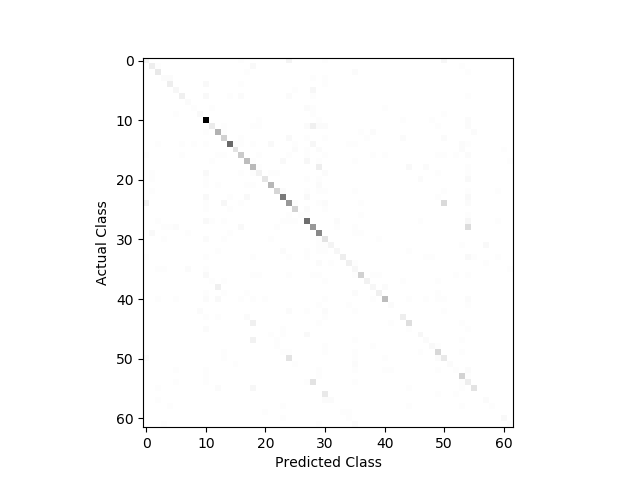
\includegraphics[scale = 0.75]{1.png}\\
From this confusion matrix, we can see that the network was able to learn the features of a few classes well enough to predict them with decent accuracy (The darker pixels in the central diagonal). \\
For some other classes, however, it learned incorrectly, and this offten missclassified the images (such as images for class 50).\\

(c) The first convolution layer is Conv2D, ie a generic 2 dimensional convoluted filter. It evolved to focus on almost all of the picture, retaining most of the features of the image.\\\\
(d) The last convolution layer is a 2D Maxpooling layer, which downsamples the image using the maximum value of each sub-region of the original image (giving an abstract version of the original image). In this network, the layer evolved to focus on the edges and the general shape of the characters in each image.
\section{Q2}
A stride is the space of pixels by which a filter moves accross an image. To explain, an example.\\
Say we have a layer with kernel size 2x2. That means that at each step, the layer takes a 2x2 pixel sample of the image and performs its operations. Now, that sample has to keep moving along the pixel grid. Here, the size of the stride steps in.\\
If the stride is, say, 1x1, then if the first sample is of (0,0) to (1,1), then the next sample will be of (0,1) to (1,2).\\
As a result, you use smalled strides when you need to capture more features of the image, and larger strides for when you need less information.

\end{document}